\section{Tempo di vita delle variabili}

\noindent Il diagramma del tempo di vita delle variabili rappresenta graficamente l'occupazione dei registri e la durata di persistenza di ogni dato all'interno del datapath durante l'esecuzione dell'algoritmo, ossia da quando viene campionato fino a quando viene utilizzato per l'ultima volta da un operando. L'asse orizzontale indica i colpi di clock, quello verticale elenca i dati in ingresso, i prodotti, le somme algebriche intermedie ed i risultati finali; il colore di ogni casella indica il registro in cui il dato è salvato.

\noindent Le parti reali dei dati di input sono presenti già al primo ciclo, per poter alimentare la prima moltiplicazione, di seguito vengono fornite le parti immaginarie. Troviamo quindi i cicli spiegati precedentemente che si sovrappongono fra loro. Inoltre, si è deciso di rappresentare l’andamento nel tempo in più iterazioni della stessa Butterfly (indicate con \#1, \#2 e \#3), quando questa lavora in modalità continua, come si può facilmente notare dalle righe del diagramma riguardanti i dati in ingresso, dove la prima occupazione di \#2 e la prima di \#1 sono distanziate da 6 colpi di clk.

\noindent Si nota che, escludendo i valori in ingresso, il numero massimo di variabili che si osservano in un ciclo è pari a 5, come si vede, ad esempio, nel ciclo 11. Per tale ragione, per non scomodare il sistema di memorizzazione degli ingressi, si è scelto di introdurre nel datapath 5 registri dediti al salvataggio dei risultati intermedi e finali, come mostrato nella sezione successiva.

\begin{figure}[H]
      \centering
      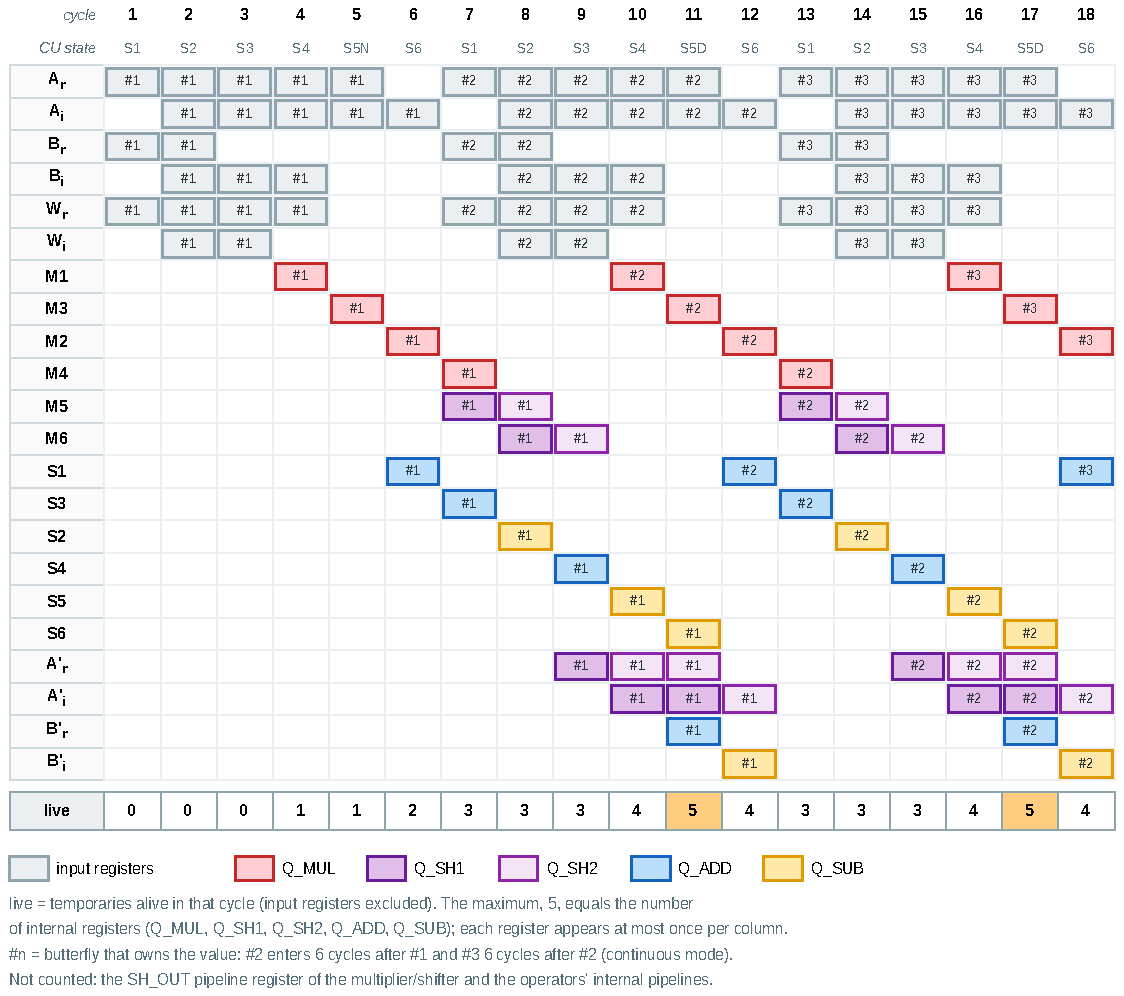
\includegraphics[width=1\textwidth]{fig11_variable_lifetime}
      \caption{Tempo di vita delle variabili}
\end{figure}
